% Stage 0b: a Verilog UART sends 'Hello world', read by the logic analyser and a serial terminal.
% Build with ./build.sh (figures, then latexmk; settings in .latexmkrc).

\documentclass[11pt,a4paper]{article}

\usepackage{fontspec}
\usepackage[margin=2.5cm]{geometry}
\usepackage{float}
\usepackage{enumitem}
\usepackage{booktabs}
\usepackage{minted}
\setminted{fontsize=\footnotesize, frame=single, framerule=0.4pt, rulecolor=black!30, framesep=4pt, xleftmargin=-8pt, xrightmargin=-8pt}
\usepackage{chapter}
\usepackage[colorlinks=true,linkcolor=blue!50!black,urlcolor=blue!50!black]{hyperref}

\setlength{\parindent}{0pt}
\setlength{\parskip}{0.6em}

\title{Hello world on the logic analyser}
\author{}
\date{}

\begin{document}
\maketitle

The logic analyser gets checked on a signal whose meaning is known before Stage~1 relies on it. The FPGA sends \texttt{Hello world} over a serial line ten times a second. The analyser decodes it; a terminal on the Mac, reading the same line through the board’s USB-serial bridge, prints it. If the two agree, the analyser, its software and the probing are right.

\section*{The serial line}

A UART sends one byte as a frame of ten bits, each lasting the same time. The line rests high. A low \emph{start} bit marks the beginning; then the eight data bits, lowest first; then a high \emph{stop} bit, after which the line can rest or the next start bit follow. Nothing marks the bits themselves: the receiver times them from the start bit’s falling edge. This is \emph{8N1}: 8 data bits, no parity, 1 stop bit.

\begin{figure}[H]
  \centering
  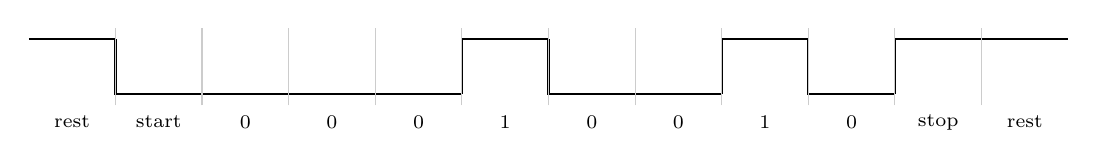
\begin{tikzpicture}[x=1.1cm, y=0.7cm]
    \foreach \v [count=\i from 0, remember=\v as \p (initially 1)] in {1,0,0,0,0,1,0,0,1,0,1,1}
      \draw[thick] (\i,\p) -- (\i,\v) -- (\i+1,\v);
    \foreach \l [count=\i from 0] in {rest, start, 0, 0, 0, 1, 0, 0, 1, 0, stop, rest}
      \node[font=\scriptsize] at (\i+0.5,-0.5) {\l};
    \foreach \i in {1,...,11}
      \draw[black!20] (\i,-0.2) -- (\i,1.2);
  \end{tikzpicture}
  \caption{The frame for \texttt{H}, \texttt{0x48} = \texttt{01001000}, sent lowest bit first.}
\end{figure}

At 115\,200 baud a bit lasts 8.68\,µs. The FPGA counts it out from its 27\,MHz clock: 27\,000\,000 / 115\,200 = 234.375, so 234 cycles per bit, which is 0.16\,\% fast. The receiver samples each bit near its middle, so errors add up along the frame: by the stop bit, ten bits in, the sample has drifted 1.6\,\% of a bit. A few per cent is fine.

\section*{Pins}

\begin{center}
\begin{tabular}{lll}
  \toprule
  Port & Pin & Goes to \\
  \midrule
  \texttt{tx} & 17 & the USB-serial bridge, so the Mac’s terminal \\
  \texttt{tx\_probe} & 19 & analyser CH0: the same signal, on a header pin \\
  \texttt{busy} & 20 & analyser CH1: high while the message goes out \\
  GND & GND & analyser GND \\
  \bottomrule
\end{tabular}
\end{center}

All three are 3.3\,V pins. \texttt{busy} is the trigger: a capture that starts on its rising edge starts on the first \texttt{H}.

\section*{The design}

\name{rtl/hello.v}:

\begin{minted}{verilog}
module hello (
    input clk,              // 27 MHz
    output tx,              // to the USB-serial bridge
    output tx_probe,        // the same, for CH0
    output reg busy = 0     // high during the message, for CH1
);

localparam BAUD = 234;                                // 27 MHz / 115200 = 234.375
localparam GAP  = 2_700_000;                          // 100 ms
localparam N    = 13;                                 // characters
localparam [8*N-1:0] MSG = {"Hello world", 8'h0d, 8'h0a};  // \r\n: Verilog has no \r

reg [9:0]  frame = 10'h3ff;  // the bits still to send, lowest first; all 1: the line rests high
reg [3:0]  left  = 0;        // bits left in this frame
reg [8:0]  baud  = 0;        // clock cycles into this bit
reg [3:0]  i     = 0;        // next character
reg [21:0] t     = 0;        // time resting between messages

assign tx = frame[0];
assign tx_probe = frame[0];

always @(posedge clk)
    if (!busy) begin                        // resting
        if (t == GAP - 1) begin
            t <= 0;
            i <= 0;
            busy <= 1;
        end else
            t <= t + 1;
    end else if (left == 0) begin           // frame done: load the next, or stop
        if (i == N)
            busy <= 0;
        else begin
            frame <= {1'b1, MSG[8*(N-1-i) +: 8], 1'b0};  // stop, data, start
            left <= 10;
            baud <= 0;
            i <= i + 1;
        end
    end else if (baud == BAUD - 1) begin    // bit done: shift in a 1, the resting level
        baud <= 0;
        frame <= {1'b1, frame[9:1]};
        left <= left - 1;
    end else
        baud <= baud + 1;

endmodule
\end{minted}

\texttt{MSG} holds the message as one 104-bit constant, first character in the top byte; \texttt{MSG[8*(N-1-i) +: 8]} picks character \texttt{i}. Each frame is loaded with its start bit at the bottom, so \texttt{tx} goes low at once, and every 234 cycles one bit moves out.

\name{constraints/hello.cst}: \texttt{clk} on 52, and \texttt{tx}, \texttt{tx\_probe}, \texttt{busy} on 17, 19 and 20, all \texttt{LVCMOS33}. Build and flash as in Stage~0a: \texttt{make flash TOP=hello}.

\section*{The terminal}

The bridge shows up on the Mac as two serial ports, one for JTAG and one for the UART:\here[which is which]

\begin{minted}{bash}
ls /dev/cu.usbserial-*
screen /dev/cu.usbserial-XXXX1 115200   # the UART; quit with Ctrl-a k
\end{minted}

\texttt{Hello world} scrolls by, ten lines a second.

\section*{The analyser}

The HiLetgo is a clone of the original Saleae Logic: 8 channels, 24 million samples a second.

\begin{enumerate}
  \item \textbf{Software.} \texttt{brew install --cask saleae-logic}, on both Macs. No driver is needed on macOS. If Logic~2 doesn’t see the device but System Information $\to$ USB lists it, the problem is in software: fall back to PulseView (\name{sigrok}, driver \name{fx2lafw}).
  \item \textbf{Probe.} GND first, to the board’s GND; CH0 to pin 19, CH1 to pin 20.
  \item \textbf{Capture.} 4\,MS/s, about 35 samples per bit, and plenty. Trigger on CH1’s rising edge; capture 2\,ms, long enough for the 13 frames (1.1\,ms).
  \item \textbf{Decode.} Add the Async Serial analyser on CH0: 115\,200 baud, 8 bits, no parity, 1 stop bit, lowest bit first.
\end{enumerate}

\textbf{Claude.} Logic~2 has an MCP server (Settings $\to$ Automation $\to$ MCP Server, experimental), which lets Claude start a capture and read the decoded text:

\begin{minted}{bash}
claude mcp add --transport http logic2 http://127.0.0.1:10530
\end{minted}

Saleae lists only its own devices as supported; whether it works with the clone is part of what this stage finds out.\here[unverified]

\section*{Done when}

The decoder reads \texttt{Hello world\textbackslash r\textbackslash n} on CH0, the terminal prints it, and Claude can start a capture and read the decoded text over the \name{logic2} MCP server.

\end{document}
